%\vspace{-0.95cm}
\subsection{Ablation Study}
\label{7.0}
\subsubsection{Parameter Efficiency}
\label{7.1}
We study how LoRA rank affects performance on DeiT-Tiny over 10 epochs. Table~\ref{tab:rank_ablation} shows performance plateaus beyond rank 8, achieving effective adaptation with only $\approx$5\% of parameters versus nearly 100\% for existing methods~\cite{shibata2021learning,adhikari2025unlearning,huang2025unified,chatterjee2024unified,liu2022continual}.
\begin{table}[!htbp]
\centering
\caption{Ablation study on the rank of LoRA modules}
\begin{tabular}{lccccc}
\toprule
Rank & \% Ratio & $Acc_f$ & $Acc_r$ & $Acc_n$ & $Acc_o$ \\
\midrule
1  & 1.09 & 1.73 & 48.57 & 27.60 & 41.58 \\
2  & 2.30 & 3.47 & 46.43 & 43.07 & 45.31 \\
4  & 3.24 & 0.00 & 65.71 & 41.87 & 57.77 \\
\rowcolor{orange!20}
8  & 5.08 & 0.80 & 76.43 & 69.60 & 74.15 \\
16 & 8.56 & 1.07 & 81.43 & 73.73 & 78.86 \\
32 & 14.80 & 0.40 & 78.57 & 76.93 & 78.03 \\
64 & 25.03 & 0.40 & 78.57 & 79.07 & 78.74 \\
\bottomrule
\end{tabular}
\label{tab:rank_ablation}
\end{table}

\subsubsection{BID-LoRA vs Standard LoRA}
\label{7.2}
As discussed in Section~\ref{4}, BID-LoRA employs distinct pathways to handle conflicting tasks like continual learning and unlearning simultaneously. Table~\ref{tab:bid_vs_standard} shows BID-LoRA outperforms standard LoRA (applied to QKV attention and classification head) in the CLU setting over 20 epochs, demonstrating that pathway separation minimizes knowledge leakage between conflicting objectives.

\begin{table}[!htbp]
\centering
\caption{BID-LoRA vs. Standard LoRA in the CLU setting}
\begin{tabular}{lccccc}
\toprule
Method & \% Ratio & $Acc_f$ & $Acc_r$ & $Acc_n$ & $Acc_o$ \\
\midrule
Standard LoRA & 2.54 & 0.00 & 74.29 & 85.07 & 77.88 \\
\rowcolor{orange!20}
BID-LoRA & 5.08 & 0.13 & 77.14 & 85.87 & 80.05 \\
\bottomrule
\end{tabular}
\label{tab:bid_vs_standard}
\end{table}

\subsubsection{Buffer Ratio}
\label{7.3}
Buffer data informs the model what to retain or forget. Here, we examine the effect of retain buffer ratio on overall accuracy. Our method is designed to remain robust even with limited buffer availability, as shown in Table.~\ref{tab:buffer_ratio}.
\begin{table}[!htbp]
\caption{Ablation on retain ratio. \textcolor{red}{$^\dagger$Rel.\ Speedup is the theoretical training-cost reduction (= 1/retain ratio), assuming cost scales linearly with buffer size; it is not a measured wall-clock time.}}
\centering
\begin{tabular}{lccccc}
\toprule
Retain Ratio & \textcolor{red}{Rel.\ Speedup$^\dagger$} & $Acc_f$ & $Acc_r$ & $Acc_n$ & $Acc_o$ \\
\midrule
1.0 & 1.0$\times$ & 0.40 & 68.00 & 81.74 & 72.58 \\
0.5 & 2.0$\times$ & 0.00 & 70.00 & 71.05 & 70.35 \\
0.3 & 3.3$\times$ & 0.00 & 66.00 & 79.11 & 70.37 \\
\rowcolor{orange!20}
0.1 & 10$\times$ & 0.00 & 65.00 & 79.96 & 69.98 \\
\bottomrule
\end{tabular}
\label{tab:buffer_ratio}
\end{table}
%\vspace{-0.74cm}
\subsubsection{Ablation on Adapters}
\label{7.4}


\begin{table}[!htbp]
\caption{Ablation on adapter pathway contributions (F=Forget, R=Retain, N=New)}
\centering
\begin{tabular}{ccc|cccc}
\toprule
F & R & N & $Acc_f$ & $Acc_r$ & $Acc_n$ & $Acc_o$ \\
\midrule
\multicolumn{3}{c|}{Pre-train} & 73.64 & 82.27 & 0.00 & 48.49 \\
\midrule
\xmark & \cmark & \cmark & 70.45 & 82.73 & 51.82 & 72.43 \\
\cmark & \xmark & \cmark & 0.00 & 0.23 & 64.55 & 21.67 \\
\rowcolor{orange!20}
\cmark & \cmark & \cmark & 0.00 & 84.09 & 56.82 & 75.00 \\
\cmark & \cmark & \xmark & 0.00 & 84.09 & 0.00 & 56.06 \\
\bottomrule
\end{tabular}
\label{tab:adapter_ablation}
\end{table}


This experiment verifies that each adapter pathway holds knowledge specific to its task. By selectively disabling pathways, we observe accuracy drops for retain and new tasks, while forget accuracy increases when its pathway is disabled. As shown in Table~\ref{tab:adapter_ablation}, the optimal performance is achieved only when all three pathways are active, validating the necessity of the tri-pathway architecture. The original classification head is restored during evaluation to isolate adapter contributions. Results are obtained over 15 epochs with pathways disabled during testing.

\subsubsection{Geometric Verification of Unlearning}
\label{7.5}
A critical question is whether forget-class embeddings actually move toward the computed escape direction $d^*$. Fig ~\ref{fig:geometric_verification}(a,b) shows t-SNE visualizations before and after unlearning. Initially, the three forget classes (0, 1, 2) are spatially separated from $d^*$. After unlearning, all three forget clusters collapse toward the dustbin point, demonstrating successful alignment with the intended escape direction.
The 3D sphere visualizations (Fig ~\ref{fig:geometric_verification} (c,d)) provide additional evidence by showing class centroids projected onto a unit sphere via PCA. While retain-class centroids (R3--R9, squares) remain anchored at their original positions relative to the retain centroid $\bar{c}_r$, the forget centroids (F0, F1, F2, circles) migrate along the antipodal axis toward $d^*$. Notably, F1 moves from a position distant from $d^*$ to near-perfect alignment after unlearning, while F0 and F2 also show substantial movement toward the escape direction. This confirms that the optimization successfully drives forget-class representations away from retain classes along the computed global escape vector.


\begin{figure}[!htbp]
    \centering
    \begin{subfigure}[b]{0.38\linewidth}
        \centering
        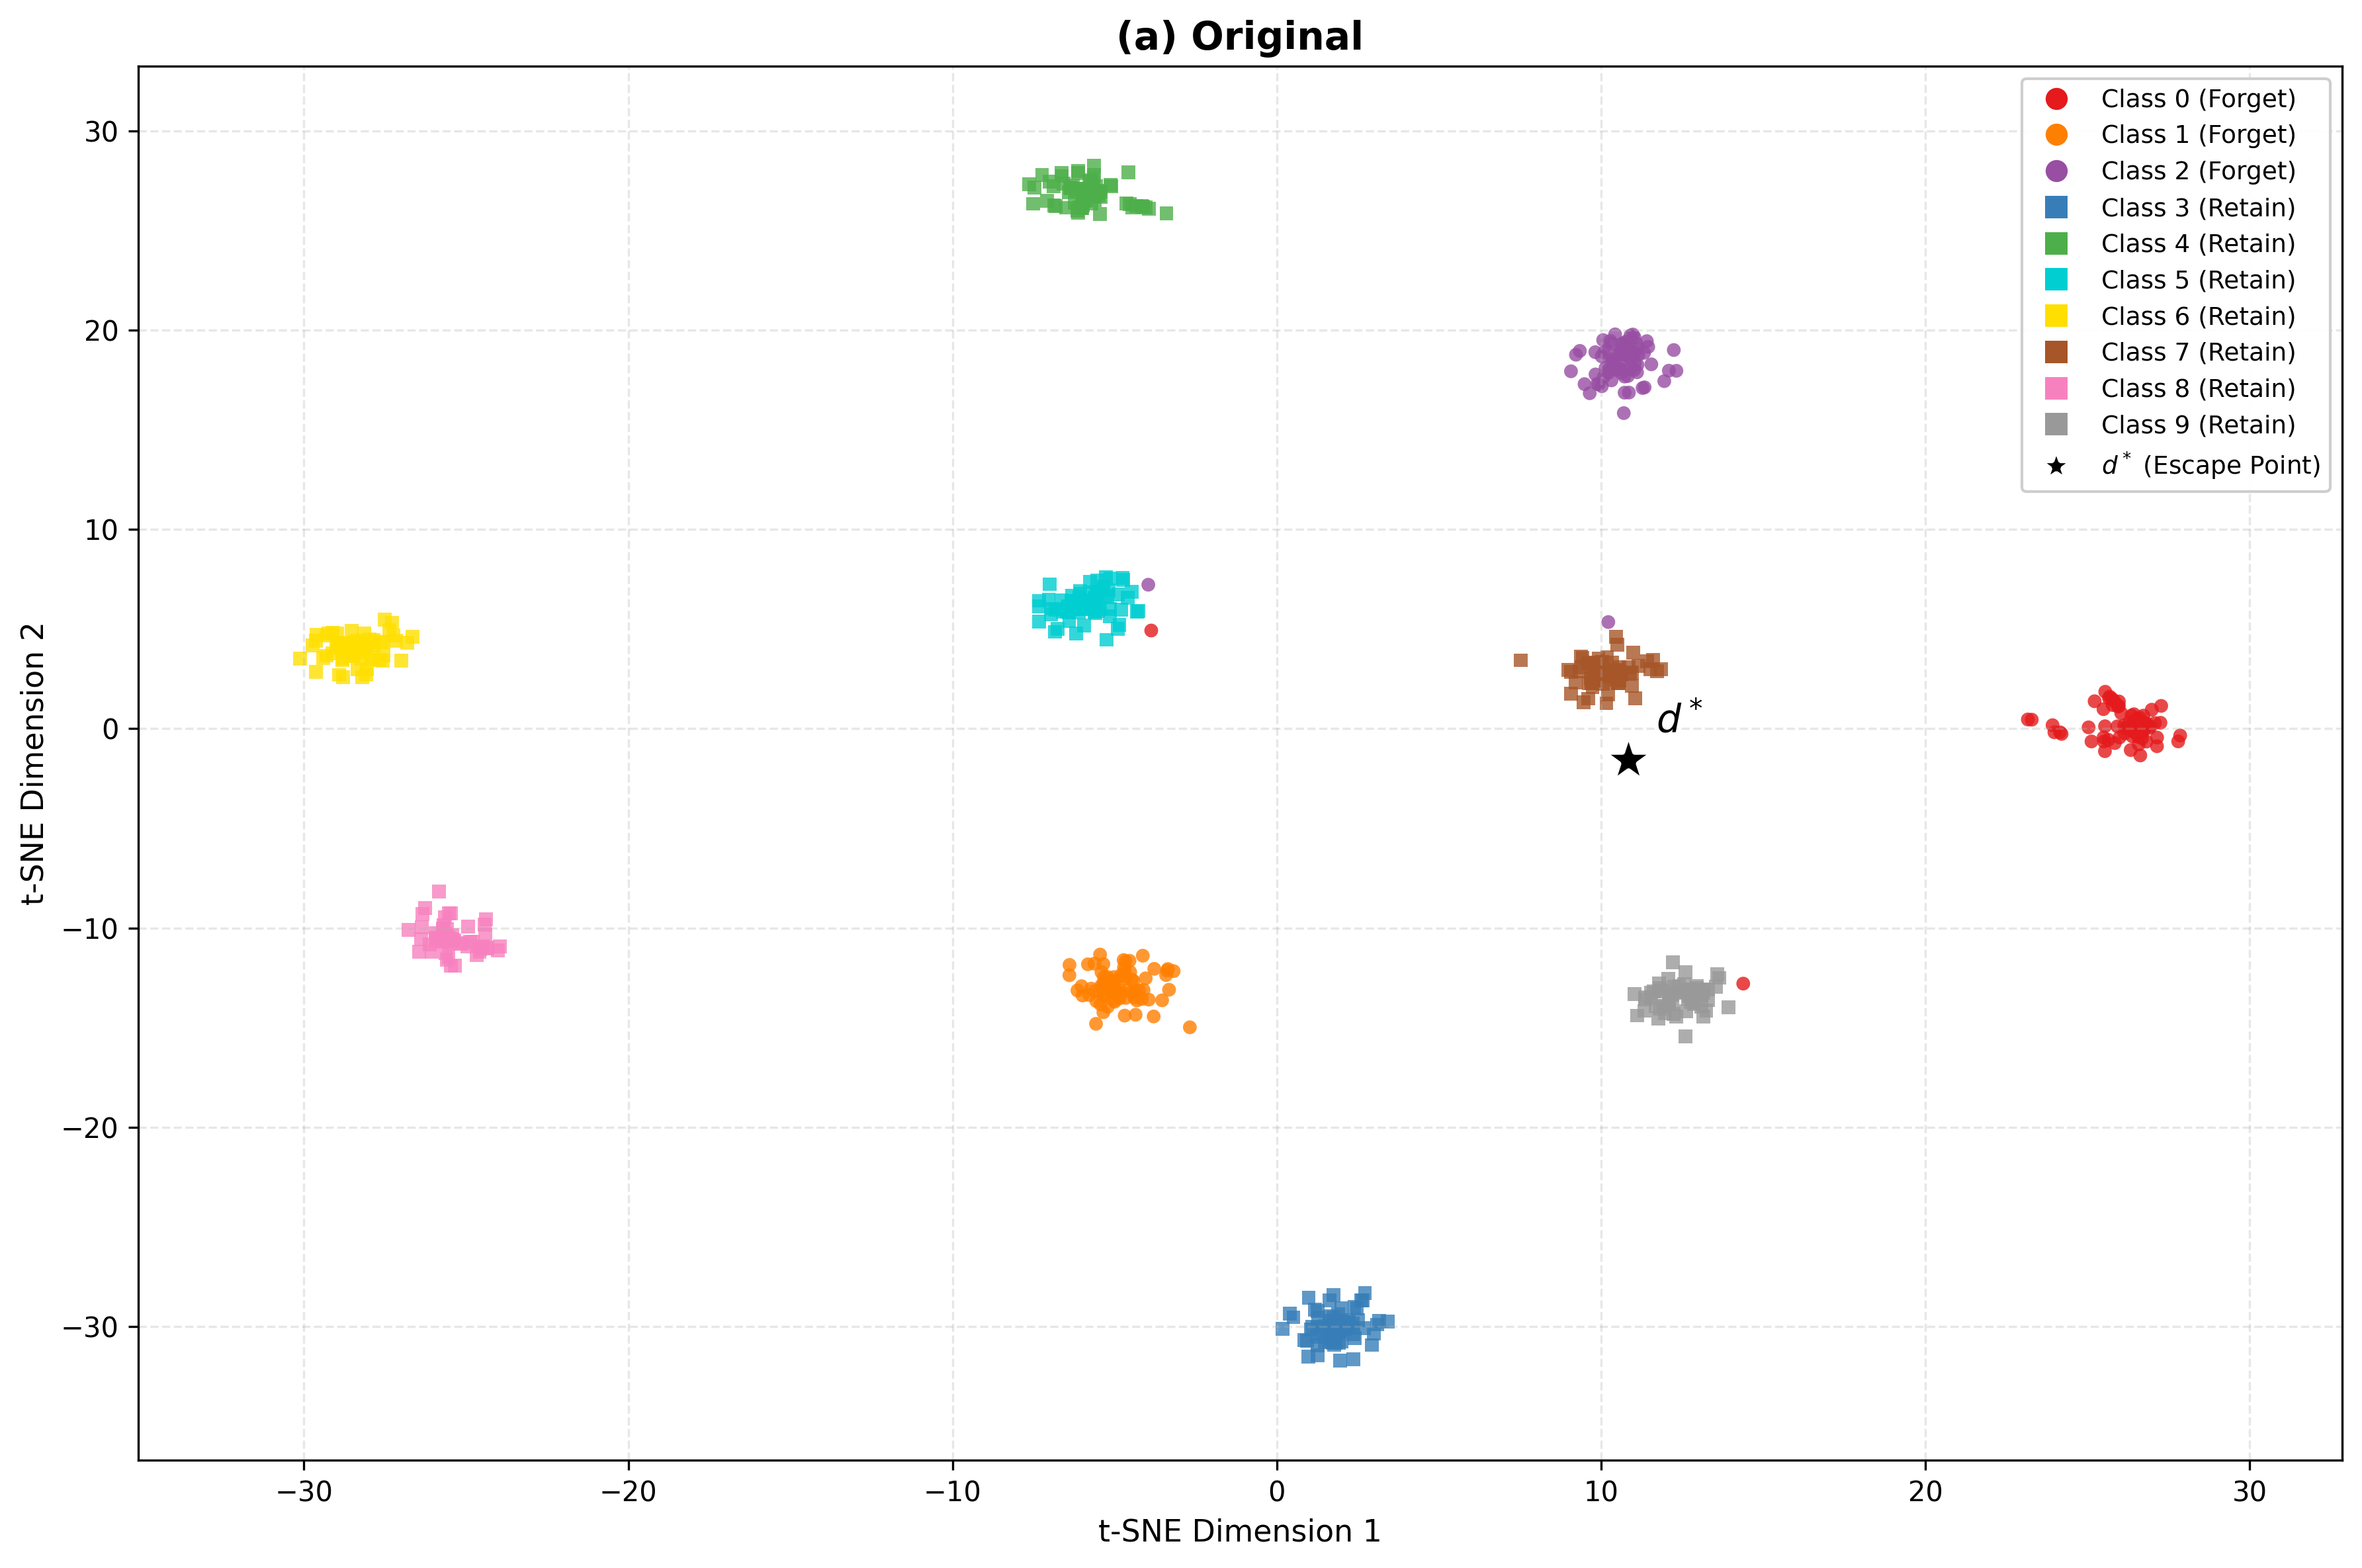
\includegraphics[width=\linewidth]{images/tsne_epoch_00.png}
        \caption{t-SNE: Before unlearning}
    \end{subfigure}
    \hspace{0.5em}
    \begin{subfigure}[b]{0.38\linewidth}
        \centering
        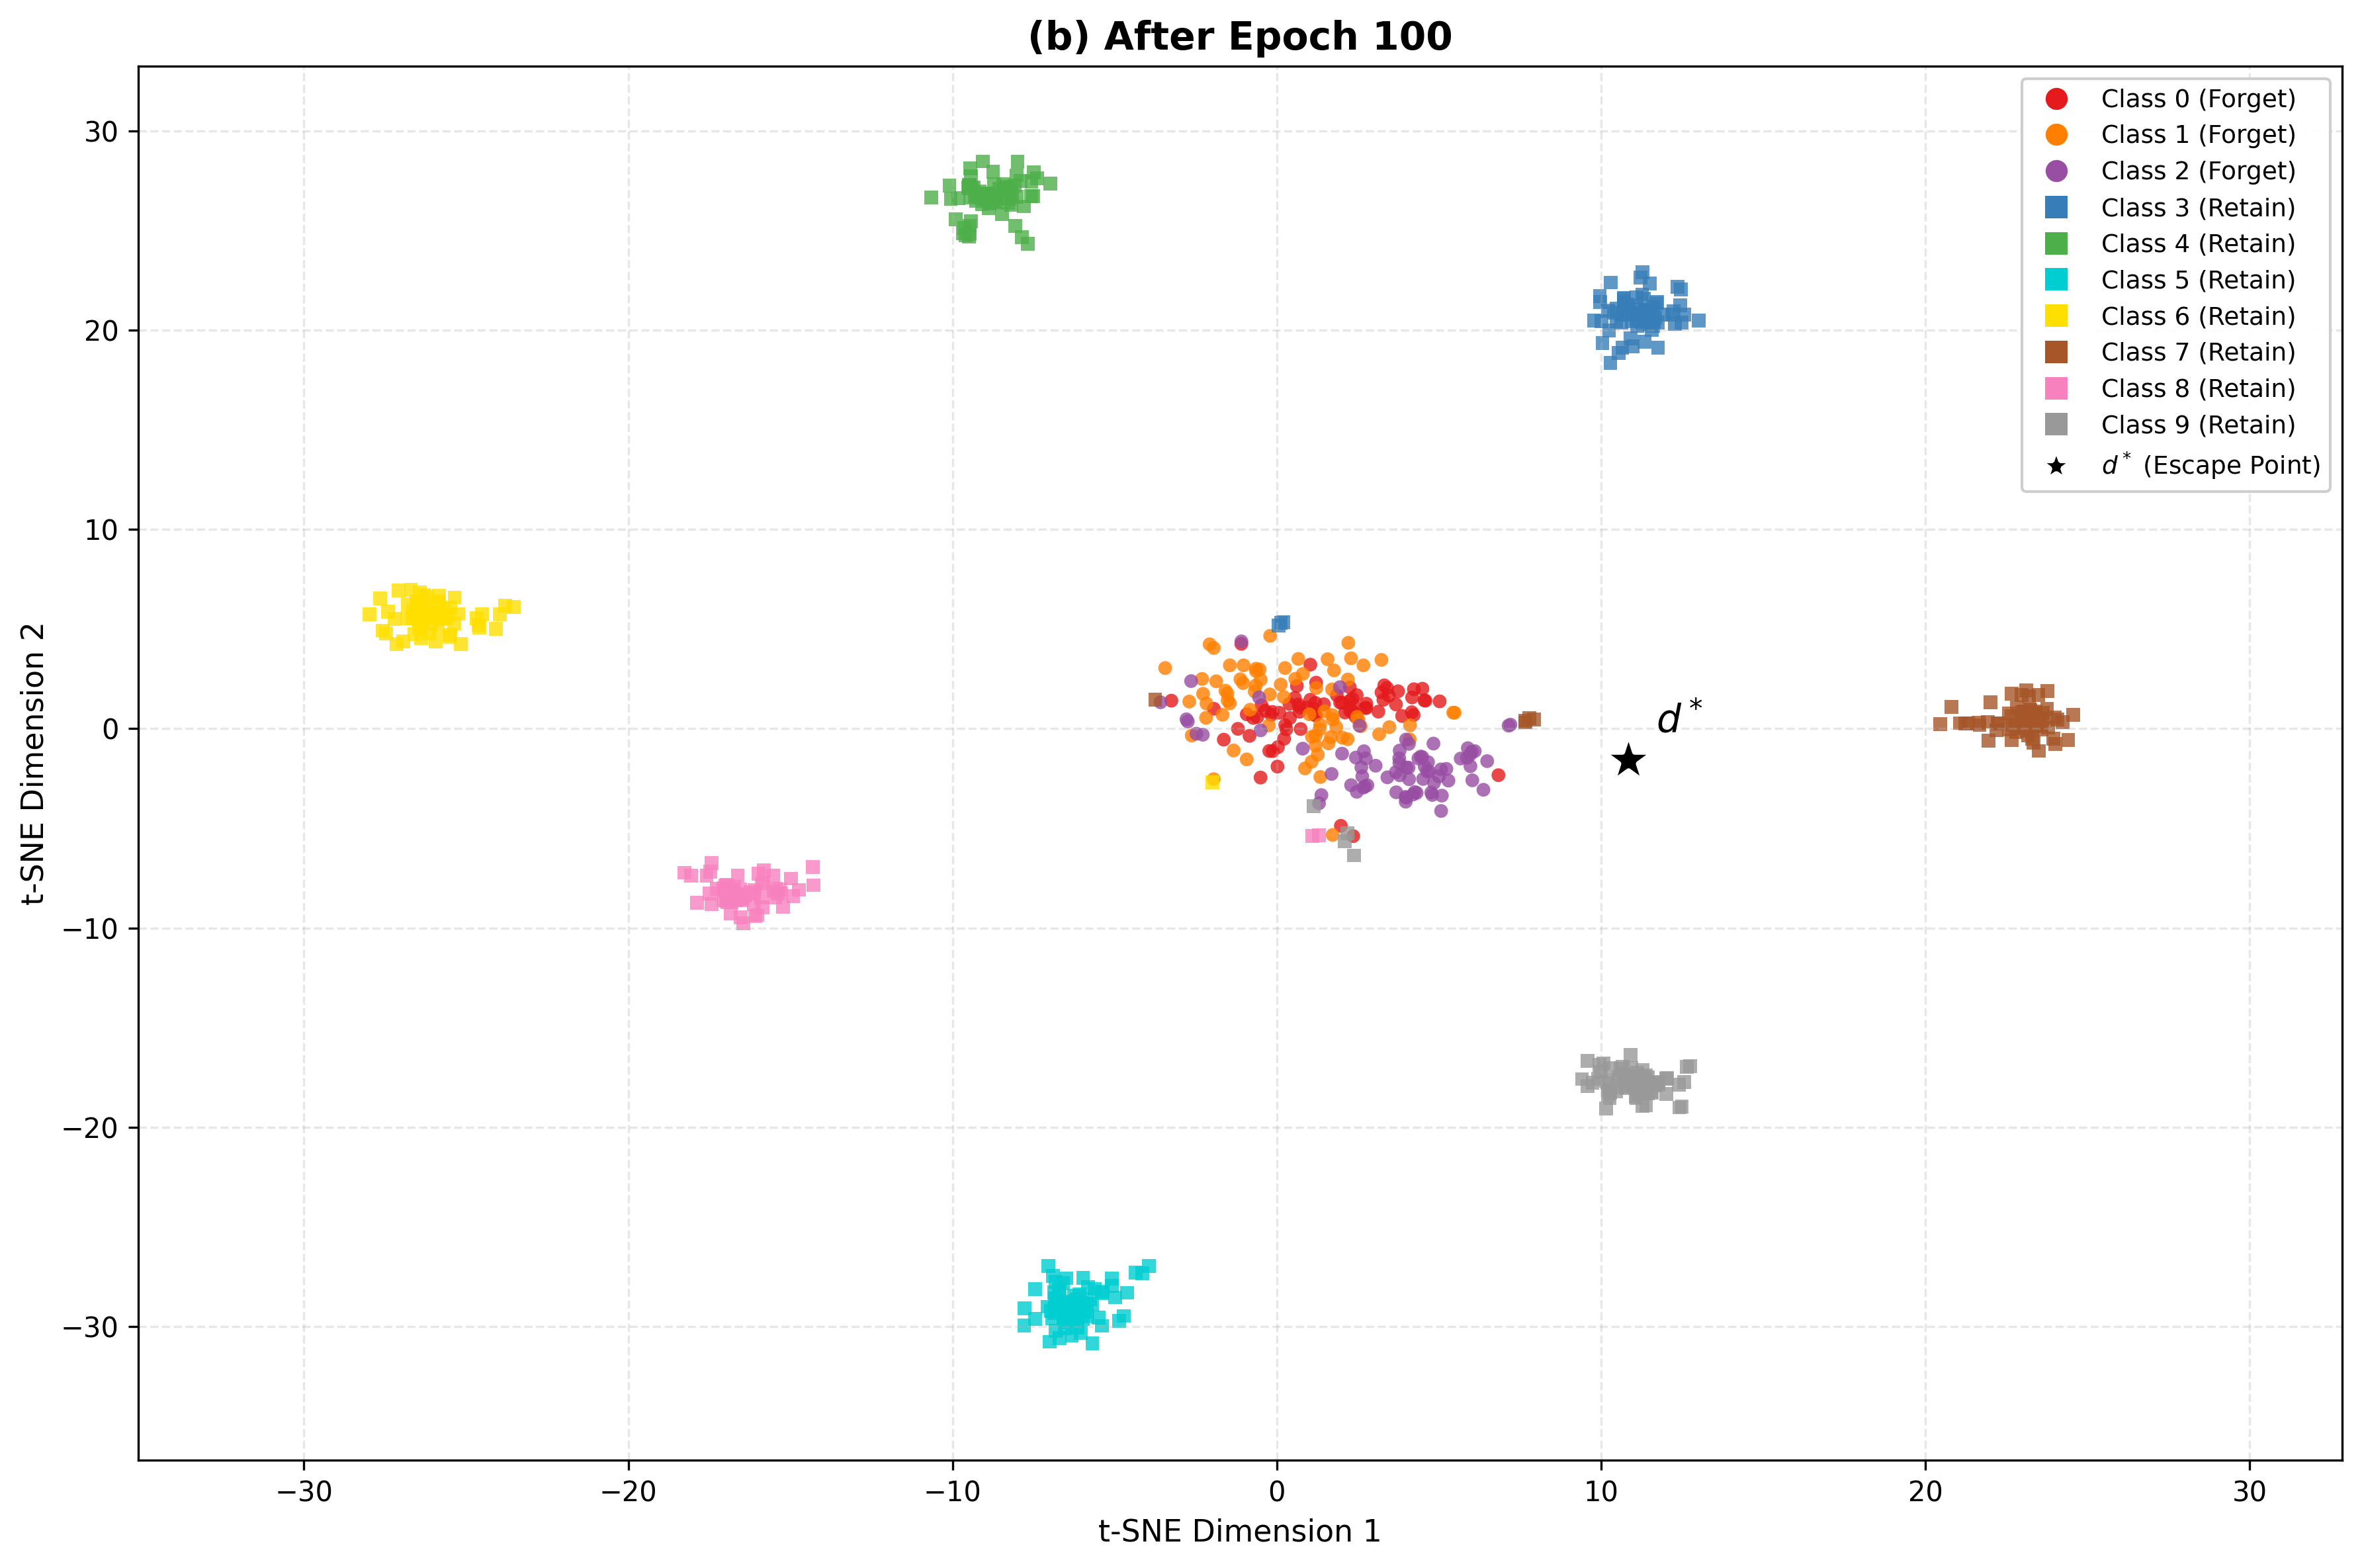
\includegraphics[width=\linewidth]{images/tsne_epoch_100.png}
        \caption{t-SNE: After unlearning}
    \end{subfigure}

    \vspace{0.8em}

    \begin{subfigure}[b]{0.38\linewidth}
        \centering
        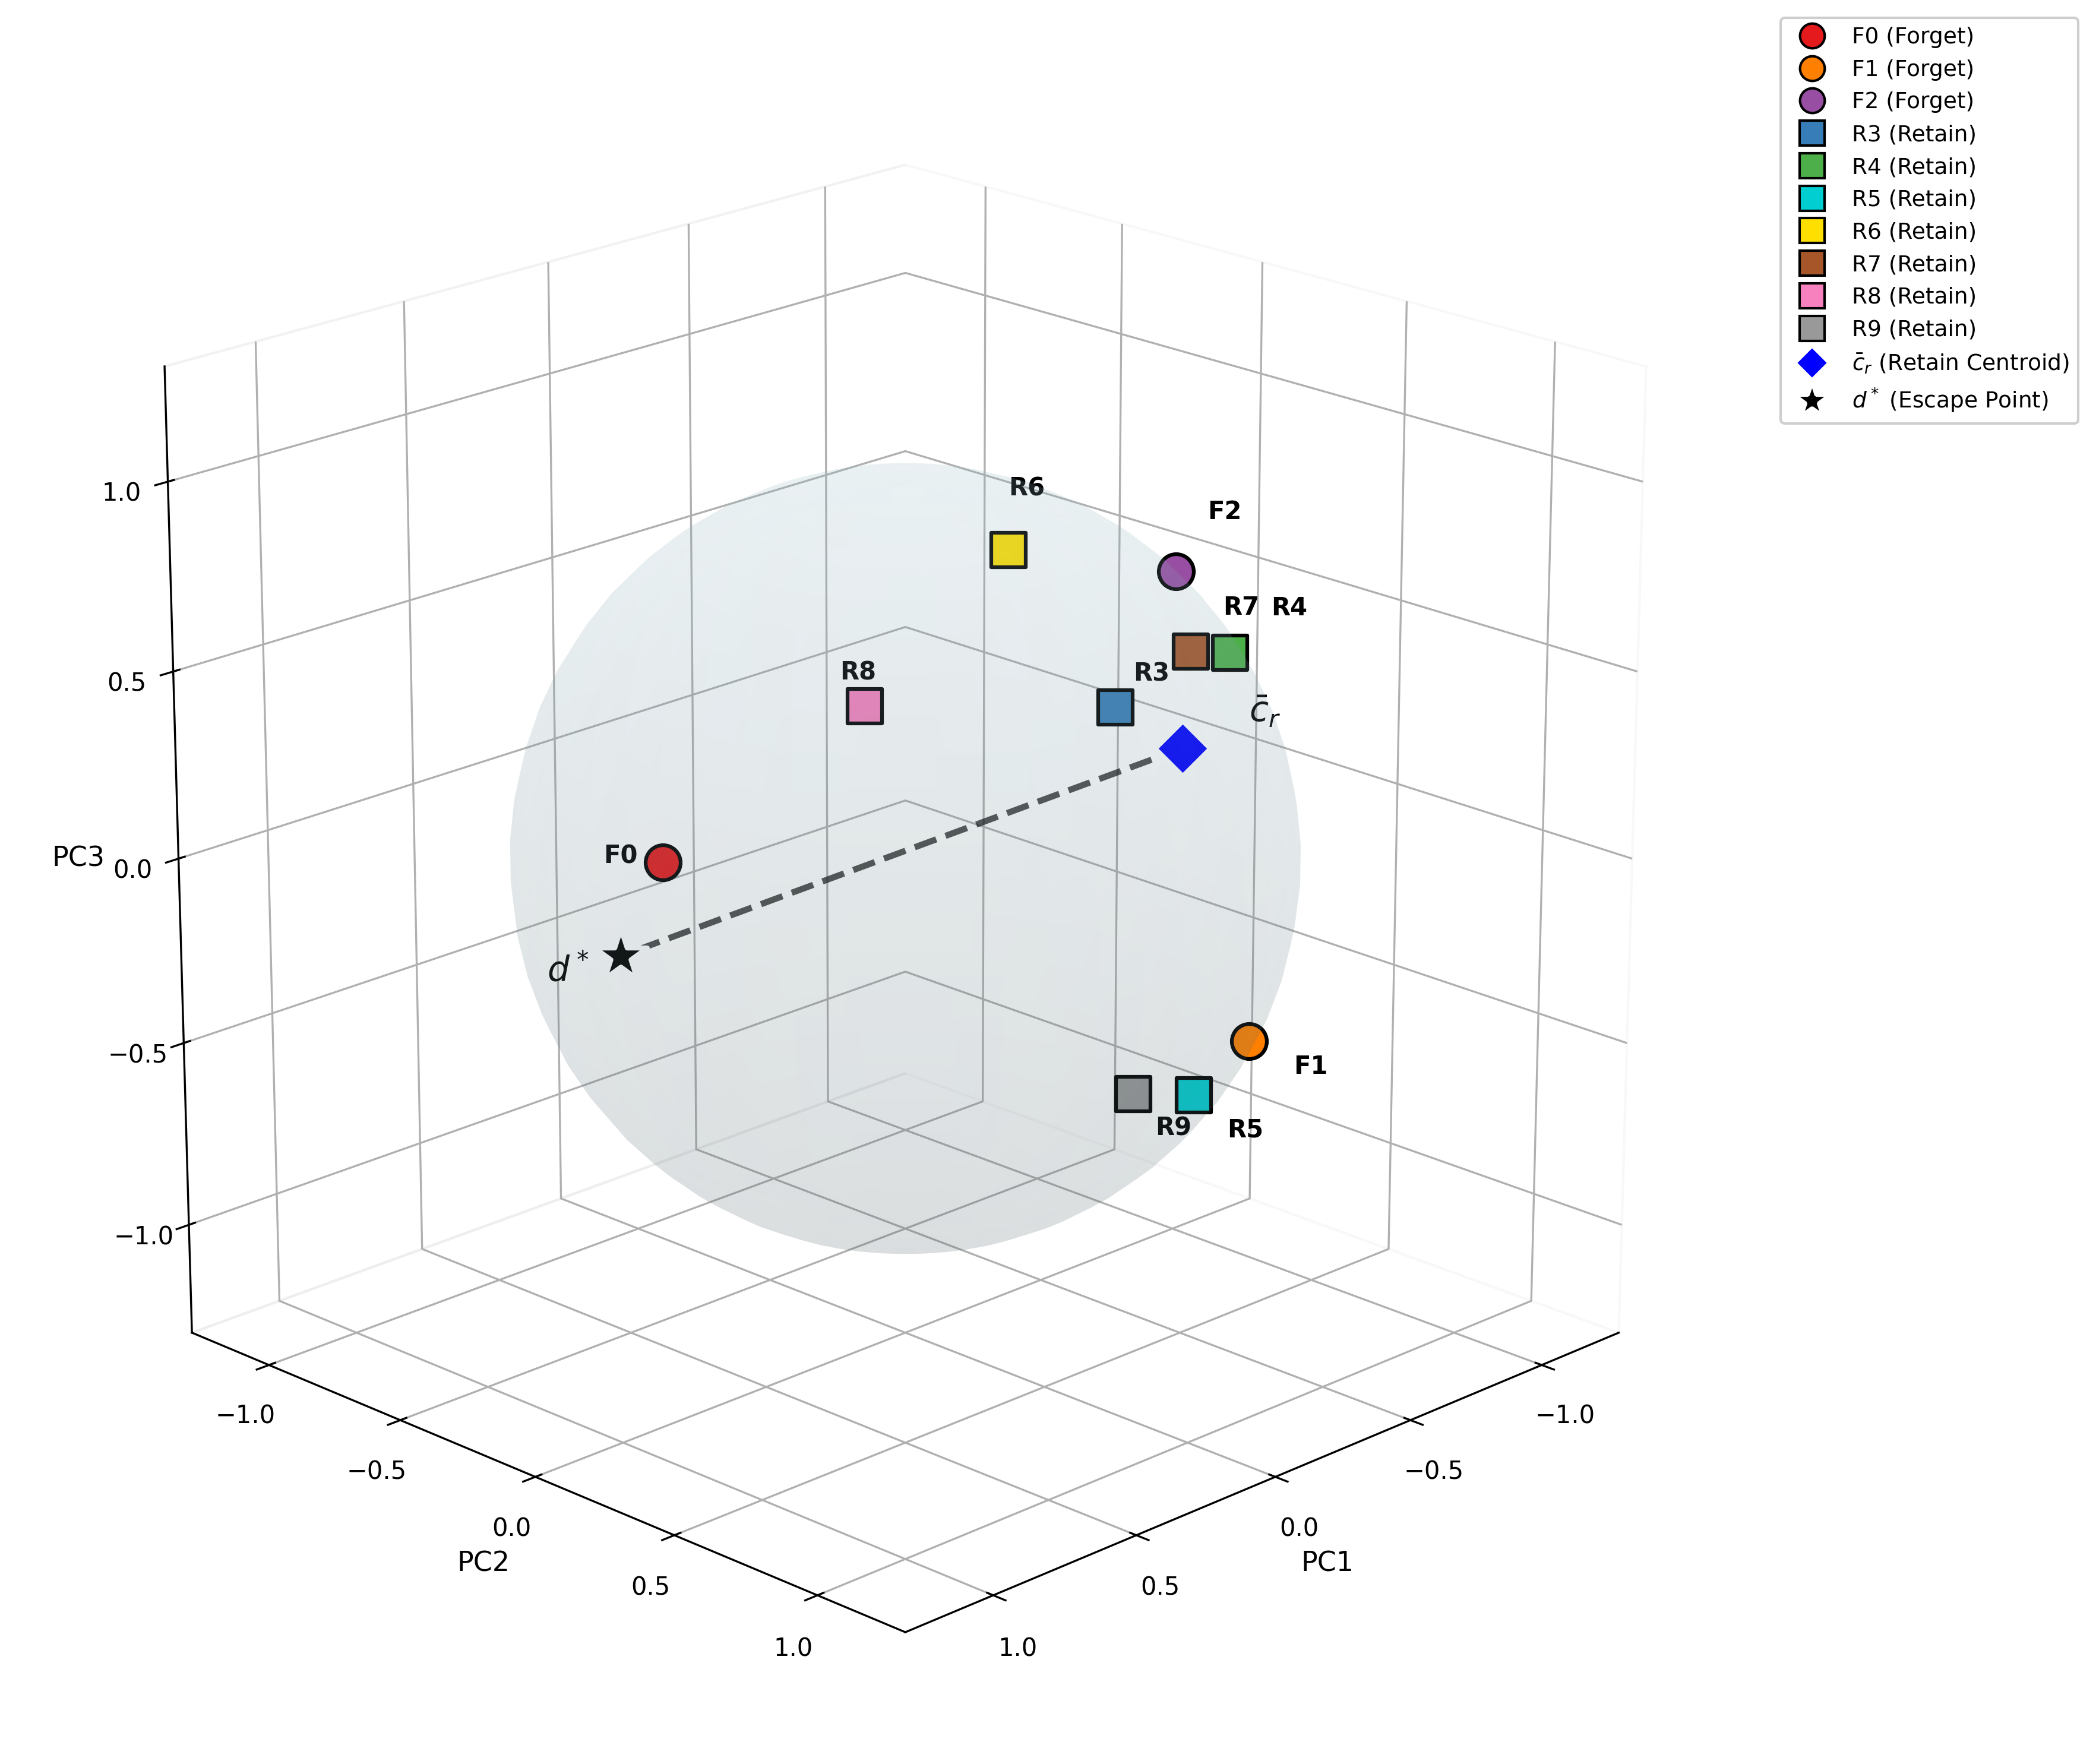
\includegraphics[width=\linewidth]{images/sphere_centroid_00.png}
        \caption{3D sphere: Before unlearning}
    \end{subfigure}
    \hspace{0.5em}
    \begin{subfigure}[b]{0.38\linewidth}
        \centering
        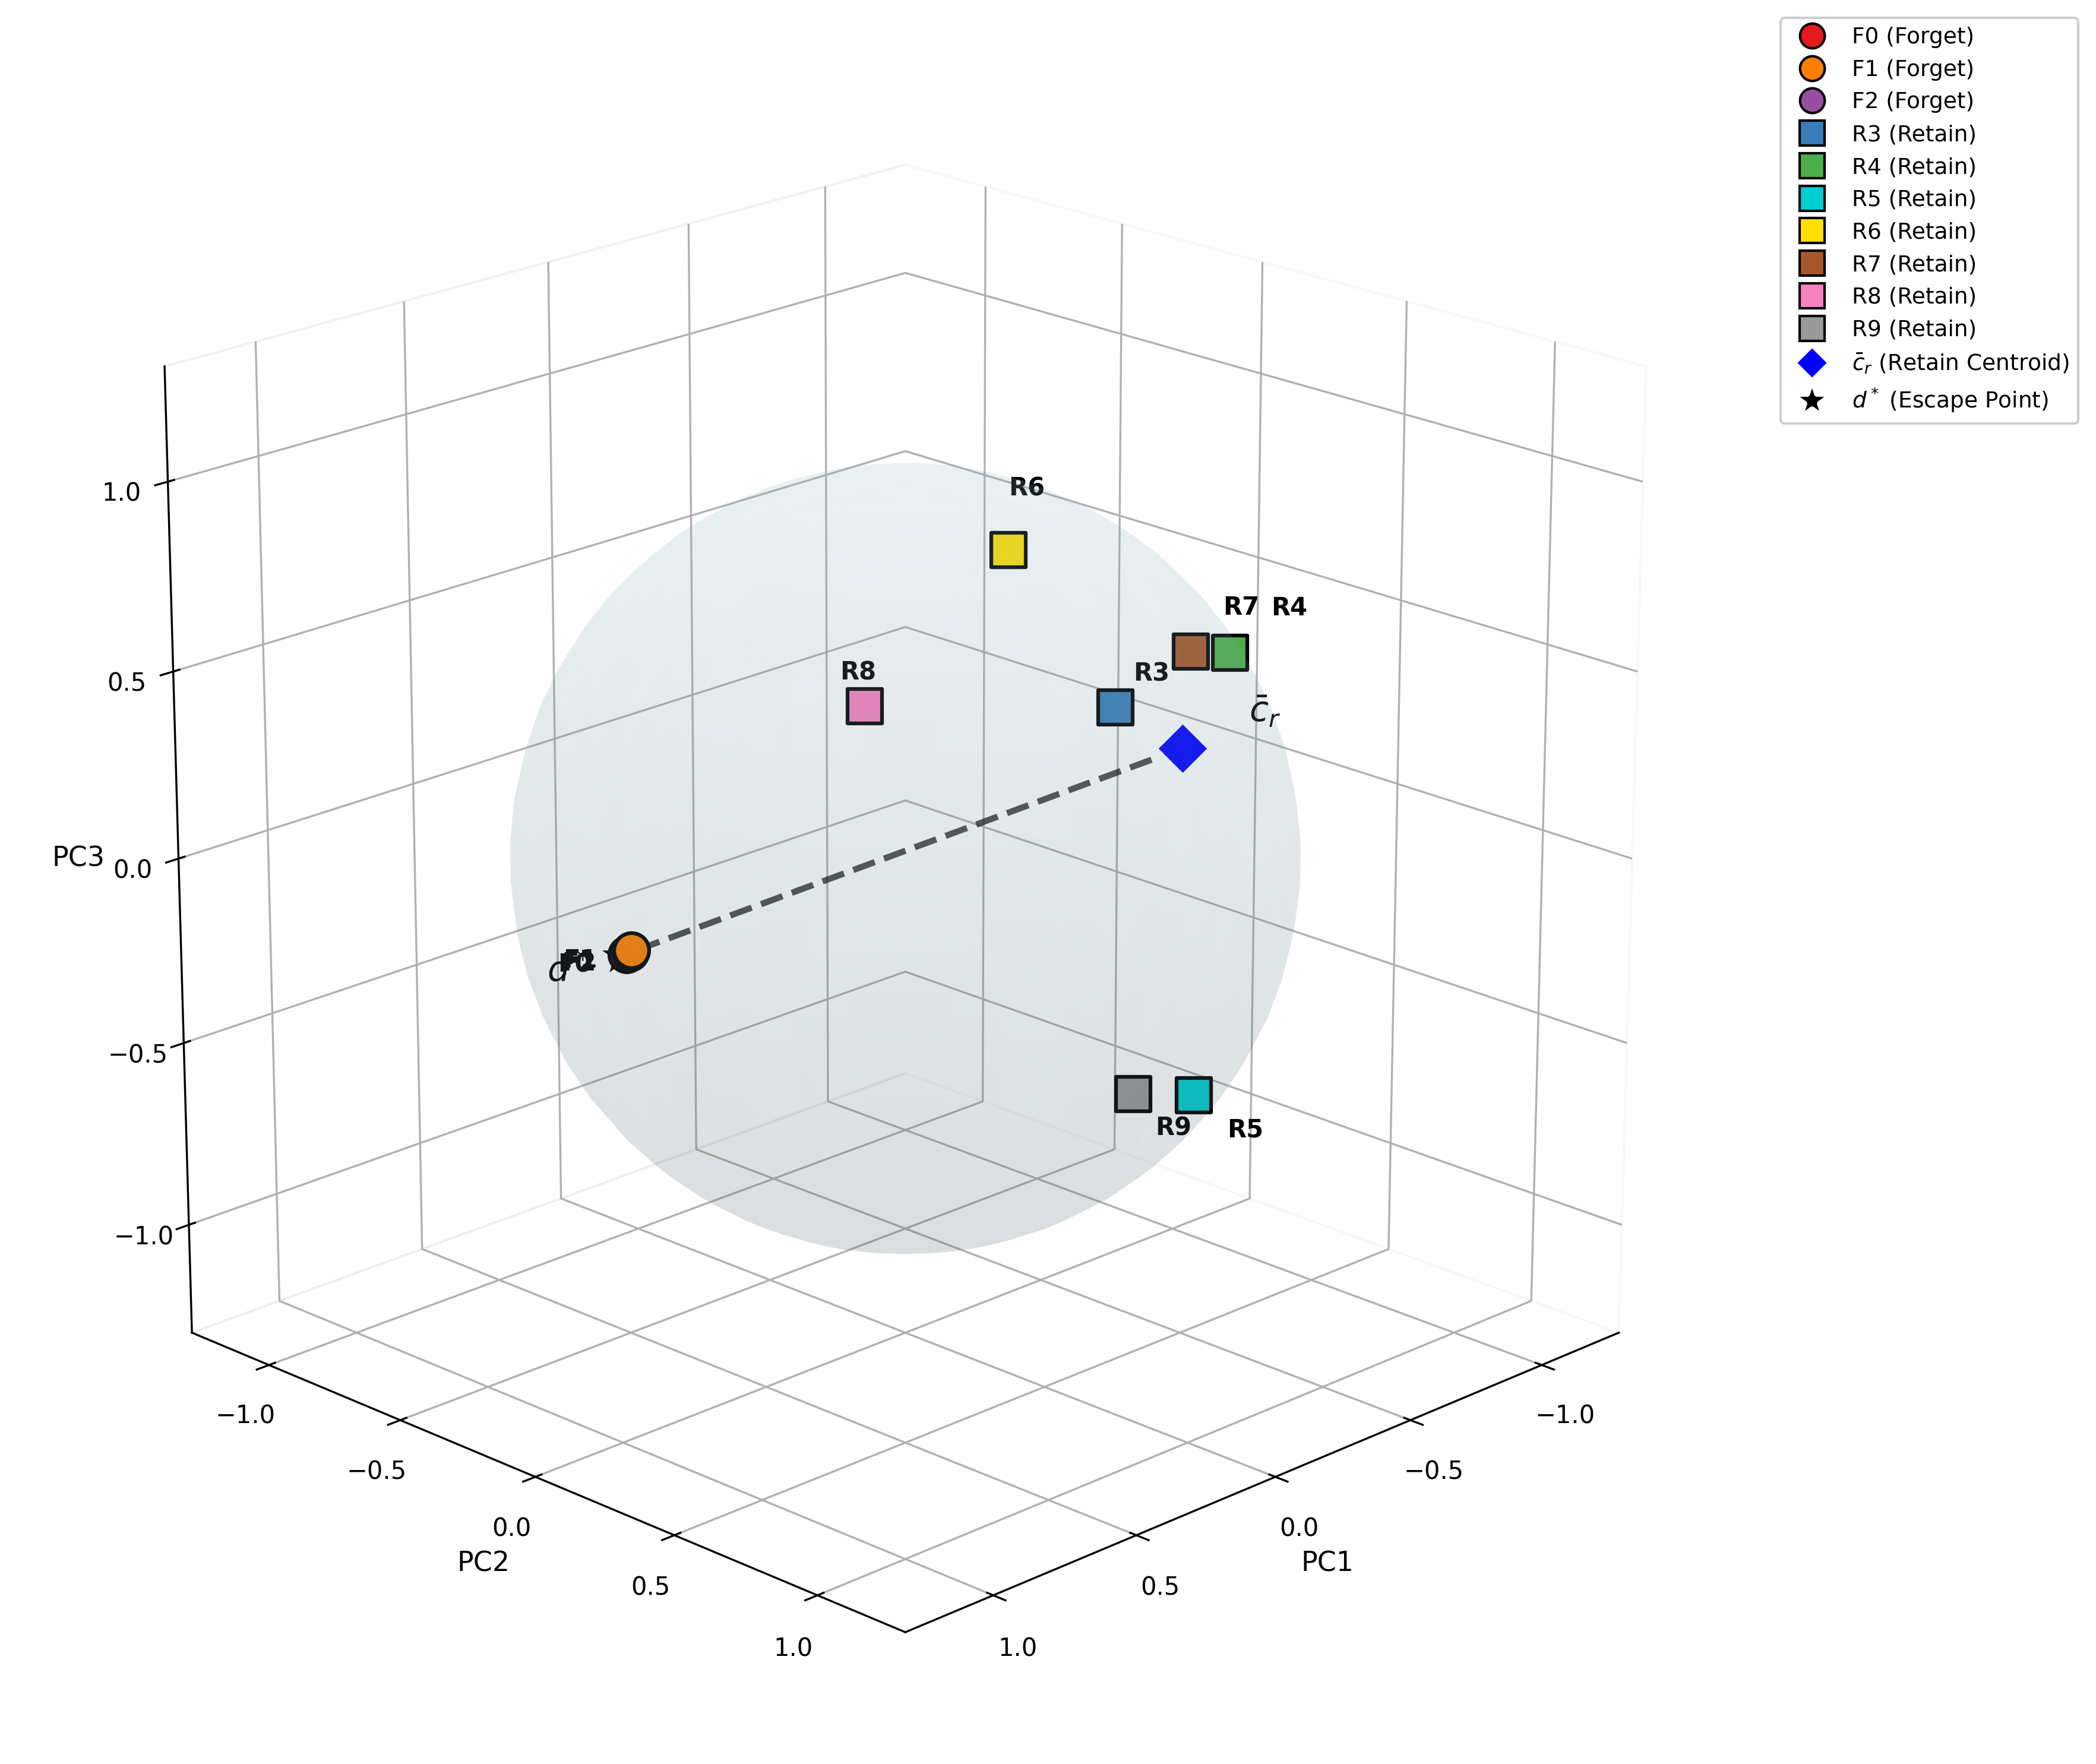
\includegraphics[width=\linewidth]{images/sphere_centroid_18.png}
        \caption{3D sphere: After unlearning}
    \end{subfigure}

    \caption{Geometric verification of unlearning. Top row: t-SNE visualization showing forget classes migrating toward escape point $d^*$. Bottom row: 3D hypersphere visualization with dashed antipodal axis from $\bar{c}_r$ to $d^*$.}
    \label{fig:geometric_verification}
\end{figure}



\subsubsection{Escape Point Scaling}
\label{7.6}
As discussed in Section~\ref{4.3}, placing $d^*$ on the unit sphere leads to unstable forgetting due to nearby centroids. Table~\ref{tab:escape_ablation} validates this: $\lambda_{\text{esc}}=10$ achieves optimal forgetting (0.53\%) by pushing the escape point beyond the embedding sphere.


% =====================================================================
% !!! PLACEHOLDER NUMBERS in tab:unlearning_evidence -- DRAFT SKELETON.
% Every value is ASSUMED. Replace with measured results before
% submission. The paragraph underneath asserts three of them
% qualitatively (Sink high, probe below Oracle, relearn ~= Oracle):
% re-check it if the measurements come out differently.
% =====================================================================

\subsubsection{\textcolor{red}{Unlearning Evidence Under Attack}}
\label{7.7}

\begin{table}[!htbp]
\centering
\footnotesize
\caption{\textcolor{red}{Unlearning evidence under attack, on the Task-6 CIFAR-100 checkpoint over all 60 classes forgotten during Tasks 1--6.}}
\label{tab:unlearning_evidence}
\textcolor{red}{
\begin{tabular}{lccc}
\toprule
\textbf{Evaluation} & \textbf{Original} & \textbf{BID-LoRA} & \textbf{Oracle} \\
                    & \textbf{(no unlearning)} & \textbf{(ours)} & \textbf{(retrain)} \\
\midrule
\multicolumn{4}{l}{\textit{Forgetting holds}} \\
\quad $Acc_f$ (cumulative, all 60 forgotten classes) $\downarrow$ & 72.91 & \textbf{0.00} & -- \\
\quad Sink: share in dominant wrong class & 4.20 & 71.34 & 14.68 \\
\midrule
\multicolumn{4}{l}{\textit{Is the information still there?}} \\
\quad Linear probe on frozen emb. (forget-class ID) $\downarrow$ & 68.53 & \textbf{8.41} & 24.77 \\
\quad Relearn @ 5-shot $\rightarrow Acc_f$ $\downarrow$ & 74.30 & \textbf{19.72} & 23.41 \\
\quad Relearn: epochs to 50\% of original $Acc_f$ $\uparrow$ & 0 & \textbf{$>$50} & $>$50 \\
\midrule
\multicolumn{4}{l}{\textit{Privacy attacks}} \\
\quad MIA, confidence-based $\approx 0.5$ & 0.78 & \textbf{0.51} & 0.50 \\
\quad MIA, label-only~\cite{choquette2021label} $\approx 0.5$ & 0.71 & \textbf{0.52} & 0.51 \\
\quad MIA, adaptive (distance to $t_{\text{escape}}$) $\approx 0.5$ & 0.50 & \textbf{0.53} & 0.50 \\
\quad Model inversion: identity match rate $\downarrow$ & 61.20 & \textbf{3.74} & 4.11 \\
\midrule
\multicolumn{4}{l}{\textit{Oracle consistency}} \\
\quad Prediction agreement with Oracle on $D_f$ $\uparrow$ & 0.12 & \textbf{0.88} & 1.00 \\
\quad KL divergence vs.\ Oracle $\downarrow$ & 3.41 & \textbf{0.79} & 0.00 \\
\bottomrule
\end{tabular}
}
\end{table}

\textcolor{red}{\emph{Original} is the pre-adaptation model and \emph{Oracle} is retrained from scratch without $D_f$, so the two bracket each attack: information present versus absent by construction. The Oracle column, not $0.5$, is therefore the target for every row, and BID-LoRA matches it on all eleven measurements. The high Sink with a probe below Oracle (chance $1/60=1.67\%$) shows collapse, not relabelling; 5-shot relearning recovers no faster than from scratch, which is what we mean by irreversible. All three MIAs use a 3-layer MLP over per-sample loss and confidence features, 5 attack initialisations, and balanced sets of 200 samples per class, with non-members drawn from held-out images of the same forgotten classes; the adaptive variant instead thresholds $\lVert \text{emb}(x)-t_{\text{escape}} \rVert$. Model inversion additionally covers class-prototype extraction, as the two share a procedure. These are empirical, attack-relative results, not a formal guarantee.}
